% ====================================
\chapter{Les tableaux à 2 dimensions}
% ====================================

% ===================
\section{Définition}
% ===================

	\marginicon{definition}
	La \textbf{dimension} d’un tableau est le nombre d’indices qu’on utilise
	pour faire référence à un de ses éléments. À ne pas confondre avec la
	taille !
	
	Dans ce qui précède, nous avons introduit les tableaux à une dimension.
	Un seul indice suffisait à localiser un de ses éléments. De nombreuses
	situations nécessitent cependant l’usage de tableaux à deux dimensions.
	Ils vous sont déjà familiers par leur présence dans beaucoup de
	situations courantes : calendrier, grille horaire, grille de mots
	croisés, sudoku, jeux se déroulant sur un quadrillage (damier,
	échiquier, scrabble, \dots).

% ====================
\section{Déclaration}
% ====================

	\marginicon{definition}
	Pour déclarer un tableau statique à 2 dimensions, on écrira :

	\cadre{
	\begin{pseudo}
	\Decl nomTableau : \K{tableau} [ ligMin à ligMax, colMin à colMax] de TypeElément
	\end{pseudo}
	}
	
	Pour un tableau dynamique, on procédera en deux étapes comme expliqué
	pour les tableaux à une dimension. On ne se permettra pas en logique de
	combiner les deux types de tableaux, à savoir utiliser la notation
	«~statique~» pour certaines dimensions et «~dynamique~» pour les
	autres.

	Notez qu'un tableau à deux dimensions peut aussi être
	vu comme un tableau à une dimension dont chacun des éléments est
	lui-même un tableau à une dimension.

	\textbf{Exemple} : Soit le tableau déclaré ainsi:

	\cadre{
	\begin{pseudo}
	\Decl ntabLettres : \K{tableau}[1 à 4, 1 à 5] de caractères
	\end{pseudo}
	}

	On peut le visualiser à l’aide d’une grille à 4 lignes et 5 colonnes.

	\begin{center}
	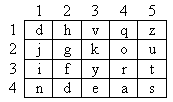
\includegraphics[width=4cm]{image/tab2d-vision-tab2d}
	\end{center}

	Ainsi, la valeur de \textstyleCodeInsr{tabLettres[3,4]} 
	est le caractère ‘r’. 
	La vision «~tableau de tableau~» 
	(ou décomposition en niveaux)
	donnerait :

	\begin{center}
	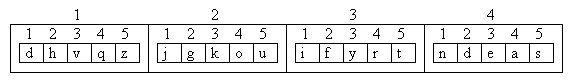
\includegraphics[width=0.9\textwidth]{image/tab2d-vision-tabtab}
	\end{center}

	Dans cette représentation, le tableau \textstyleCodeInsr{tabLettres} est
	d’abord décomposé à un premier niveau en quatre éléments auxquels on
	accède par le premier indice. Ensuite, chaque élément de premier niveau
	est décomposé en cinq éléments de deuxième niveau accessibles par le
	deuxième indice.

% ============================================
\section{La troisième dimension (et au-delà)}
% ============================================

	Certaines situations complexes nécessitent l'usage de
	tableaux à 3 voire plus de dimensions.

	\marginicon{definition}
	Pour déclarer un tableau statique à k dimensions, on écrira :

	\cadre{
	\begin{pseudo}
	\Decl nomTableau : \K{tableau} [ bMin\_1 à bMax\_1, \dots, bMin\_k à bMax\_k] de TypeElément
	\end{pseudo}
	}

	où chaque paire de bornes \textstyleCodeInsr{bMin\_i}~et
	\textstyleCodeInsr{bMax\_i} limite l’indice correspondant à la ième
	dimension du tableau.

% ===================
\section{ Exercices}
% ===================

\begin{Exercice}{Affichage}
	Écrire un module qui affiche tous les éléments d'un
	tableau à n lignes et m colonnes
	\begin{enumerate}[label=\alph*)]
	\item ligne par ligne ;
	\item colonne par colonne.
	\end{enumerate}
\end{Exercice}

\begin{Exercice}{Les nuls}
	\marginicon{java}
	Écrire un module qui reçoit un tableau (n x m)
	d'entiers et qui affiche la proportion
	d'éléments nuls dans ce tableau.
\end{Exercice}

\begin{Exercice}{Le contour du tableau}
	\marginicon{java}
	On donne un tableau d’entiers tabEnt à n lignes et m colonnes. 
	Écrire un module retournant la somme 
	de tous les éléments \textit{impairs}
	situés sur le bord du tableau.

	Exemple : pour le tableau suivant, le module doit renvoyer $32$

	\begin{center}
	\begin{tabular}{|*{4}{>{\centering\arraybackslash}m{0.6cm}|}}
	  \hline
	  3 & 4 & 6 & 11\\\hline
	  2 & 21 & 7 & 9\\\hline
	  1 & 5 & 12 & 3\\\hline
	\end{tabular}
	\end{center}

	Et pour le suivant, le module doit renvoyer $6$

	\begin{center}
	\begin{tabular}{|*{5}{>{\centering\arraybackslash}m{0.3cm}|}}
	\hline
	 4 & 1 & 2 & 8 & 5\\\hline
	\end{tabular}
	\end{center}
\end{Exercice}

\begin{Exercice}{À vos pinceaux !}
	On possède un tableau à n lignes et n colonnes dont les éléments de type
	Couleur valent NOIR ou BLANC. On suppose que le tableau est initialisé
	à ‘BLANC’ au départ. Écrire un module qui ‘noircit’ les cases de ce
	tableau comme le suggèrent les dessins suivants~(les exemples sont
	donnés pour un tableau 10 x 10 mais les algorithmes doivent fonctionner
	quelle que soit la taille du tableau).
	
	\begin{center}
	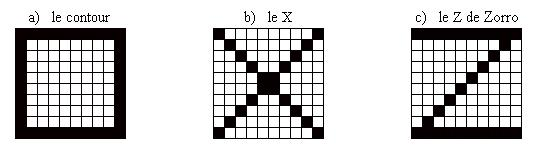
\includegraphics[width=0.9\textwidth]{image/tab2d-ex-oxz}
	\end{center}
\end{Exercice}

\begin{Exercice}{Le tableau de cotes}
	Soit un tableau à n lignes et m colonnes d'entiers où
	une ligne représente les notes sur 20 d'un étudiant et
	les colonnes toutes les notes d'un cours.
	
	Écrire un algorithme recevant ce tableau en paramètre et affichant le
	pourcentage d'étudiants ayant obtenu une moyenne
	supérieure à 50\%.
\end{Exercice}

\begin{Exercice}{Tous positifs}
	\marginicon{java}
	Écrire un module qui reçoit un tableau (n x m) d’entiers et qui vérifie
	si tous les nombres qu’il contient sont strictement positifs. Bien sûr,
	on veillera à éviter tout travail inutile; la rencontre d’un nombre
	négatif doit arrêter le module.
\end{Exercice}

\begin{Exercice}{Le carré magique}
	\marginicon{java}
	Un carré magique est un tableau d’entiers carré
	(c'est-à-dire possédant autant de lignes que de
	colonnes) ayant la propriété suivante: si on additionne les éléments
	d'une quelconque de ses lignes, de ses colonnes ou de
	ses deux diagonales, on obtient à chaque fois le même résultat.

	Écrire un module recevant en paramètres le tableau[1 à n, 1 à n]
	d'entiers Carré et renvoyant une valeur booléenne
	indiquant si Carré est un carré magique ou non.
\end{Exercice}

\begin{Exercice}{Le triangle de Pascal}
	Le triangle de Pascal est construit de la façon suivante :

	\begin{itemize}
	\item la ligne initiale contient un seul élément de valeur 1 ;
	\item chaque ligne possède un élément de plus que la précédente ;
	\item chaque ligne commence et se termine par 1 ;
	\item 
		pour calculer un nombre d’une autre case du tableau, on additionne le
		nombre situé dans la case située juste au-dessus avec celui dans la
		case à la gauche de la précédente.
	\end{itemize}

	Écrire un module qui reçoit en paramètre un entier
	\textstyleCodeInsr{n}, et qui renvoie un tableau contenant les
	\textstyleCodeInsr{n+1} premières lignes du triangle de Pascal
	(indicées de \textstyleCodeInsr{0} à \textstyleCodeInsr{n}).
	N.B.: le «~triangle~» sera bien entendu renvoyé dans un tableau carré.
	Quid des cases non occupées ?

	Par exemple, pour n = 5, on aura le tableau suivant :

	\begin{center}
	\begin{tabular}{|*{6}{>{\centering\arraybackslash}m{0.33cm}|}}
	\hline
	 1 & ~ & ~ & ~ & ~ & ~ \\\hline
	 1 & 1 & ~ & ~ & ~ & ~ \\\hline
	 1 & 2 & 1 & ~ & ~ & ~ \\\hline
	 1 & 3 & 3 & 1 & ~ & ~ \\\hline
	 1 & 4 & 6 & 4 & 1 & ~ \\\hline
	 1 & 5 & 10 & 10 & 5 & 1 \\\hline
	\end{tabular}
	\end{center}
\end{Exercice}

\begin{Exercice}{Le calendrier du mois}
	Écrire un module qui reçoit en paramètres 
	le numéro du premier jour du mois 
	(c-à-d 1 si le mois commence un lundi, 2 si le mois commence un mardi,
	etc.) ainsi que le nombre de jours dans le mois.
	Au départ de ces données, 
	le module remplira avec les dates des jours du mois un tableau
	«~calendrier~» à deux dimensions, 
	dont les colonnes représentent les jours 
	(la première colonne correspondant au lundi) et les lignes les
	semaines. 
	Par exemple, si le mois contient 30 jours et le premier jour
	est un mercredi, le contenu du tableau sera :

	\begin{center}
	\tablehead{}
	\begin{supertabular}{|m{0.807cm}|m{0.807cm}|m{0.807cm}|m{0.807cm}|m{0.807cm}|m{0.807cm}|m{0.81100005cm}|}
	\multicolumn{1}{m{0.807cm}}{\centering 
	\textstylePolicepardfauti{L}} &
	\multicolumn{1}{m{0.807cm}}{\centering 
	\textstylePolicepardfauti{M}} &
	\multicolumn{1}{m{0.807cm}}{\centering 
	\textstylePolicepardfauti{M}} &
	\multicolumn{1}{m{0.807cm}}{\centering 
	\textstylePolicepardfauti{{J}}} &
	\multicolumn{1}{m{0.807cm}}{\centering 
	\textstylePolicepardfauti{{V}}} &
	\multicolumn{1}{m{0.807cm}}{\centering 
	\textstylePolicepardfauti{{S}}} &
	\multicolumn{1}{m{0.81100005cm}}{\centering\arraybslash
	 \textstylePolicepardfauti{D}}\\\hline
	~
	 &
	~
	 &
	\raggedleft  \textstylePolicepardfauti{1} &
	\raggedleft  \textstylePolicepardfauti{2} &
	\raggedleft  \textstylePolicepardfauti{3} &
	\raggedleft  \textstylePolicepardfauti{4} &
	\raggedleft\arraybslash 
	\textstylePolicepardfauti{5}\\\hline
	\raggedleft  \textstylePolicepardfauti{6} &
	\raggedleft  \textstylePolicepardfauti{7} &
	\raggedleft  \textstylePolicepardfauti{8} &
	\raggedleft  \textstylePolicepardfauti{9} &
	\raggedleft  \textstylePolicepardfauti{10} &
	\raggedleft  \textstylePolicepardfauti{11} &
	\raggedleft\arraybslash 
	\textstylePolicepardfauti{12}\\\hline
	\raggedleft  \textstylePolicepardfauti{13} &
	\raggedleft  \textstylePolicepardfauti{14} &
	\raggedleft  \textstylePolicepardfauti{15} &
	\raggedleft  \textstylePolicepardfauti{16} &
	\raggedleft  \textstylePolicepardfauti{17} &
	\raggedleft  \textstylePolicepardfauti{18} &
	\raggedleft\arraybslash 
	\textstylePolicepardfauti{19}\\\hline
	\raggedleft  \textstylePolicepardfauti{20} &
	\raggedleft  \textstylePolicepardfauti{21} &
	\raggedleft  \textstylePolicepardfauti{22} &
	\raggedleft  \textstylePolicepardfauti{23} &
	\raggedleft  \textstylePolicepardfauti{24} &
	\raggedleft  \textstylePolicepardfauti{25} &
	\raggedleft\arraybslash 
	\textstylePolicepardfauti{26}\\\hline
	\raggedleft  \textstylePolicepardfauti{27} &
	\raggedleft  \textstylePolicepardfauti{28} &
	\raggedleft  \textstylePolicepardfauti{29} &
	\raggedleft  \textstylePolicepardfauti{30} &
	~
	 &
	~
	 &
	~
	\\\hline
	\end{supertabular}
	\end{center}

	\textbf{Réflexions} :

	\begin{itemize}
	\item Combien de lignes au maximum doit avoir ce tableau ?
	\item Quid des cases non occupées ?
	\end{itemize}
\end{Exercice}

\begin{Exercice}{À vos pinceaux (la suite) !}
	Pour poursuivre l'exercice du pinceau, 
	voici quelques cas plus coriaces.
	
	\begin{center}
	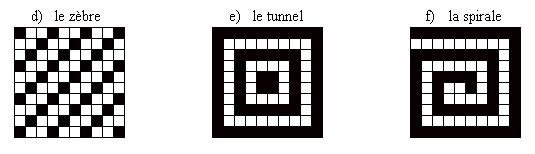
\includegraphics[width=0.9\textwidth]{image/tab2d-ex-zts}
	\end{center}
\end{Exercice}

\begin{Exercice}{Exercices sur la complexité}

	\begin{enumerate}[label=\alph*)]
	\item 
		Quelle est la complexité d’un algorithme de parcours
		d'un tableau n x n ?
	\item
		Et pour un algorithme qui remet à 0 toutes les
		occurrences du maximum d'un tableau n x n ?
	\item 
		Quelle est la complexité de
		l'algorithme que vous avez écrit pour résoudre les
		exercices du pinceau ?
	\end{enumerate}
\end{Exercice}

\begin{Exercice}{Lignes et colonnes}
	Écrire un module qui reçoit un tableau d’entiers à 2 dimensions en paramètre 
	et qui retourne un booléen indiquant si ce tableau 
	possède 2 lignes ou 2 colonnes identiques.
	
	Dans l’affirmative, 
	ce module renverra également en paramètres les informations suivantes :
	
	\begin{itemize}
	\item les indices des lignes ou colonnes identiques
	\item un caractère valant ‘L’ ou ‘C’ selon qu’il s’agit de lignes ou de
	colonnes
	\end{itemize}
	
	Dans la négative, les valeurs de ces paramètres seront indéterminées ou
	quelconques, elles ne seront de toute façon pas utilisées par le module
	appelant.
\end{Exercice}
